%TODO: add list of benchmarks, each with explanation and charactaristics.
%Add picture of complete toolflow (from C to estimates).
%Add results section,
%Add discussion on results

In order to evaluate the performance of the compiler, a set of benchmarks is used. The assembly code generated by the two compilers will be compared on `code quality' and on the number of register reads and writes it can avoid by exploiting explicit datapaths. To verify correctness of the generated code, the simulation output of the code generated by the LLVM compiler and of the code produced by the legacy compiler are compared to a reference. The references are generated using GCC\footnote{gcc.gnu.org} and the result of GCC is an executable that prints the reference output upon execution. This reference output is compared to the simulation results and if they match, the compiler can generate a correct code.

To compare the two compilers, scalar-only code is considered such that the comparison is fair. Then the auto-vectorizer is enabled for further analysis which results in more efficient code. This in turn is compared to handwritten assembly code to see how efficient the generated code truly is.

\section{Benchmarks}
The collection of benchmarks is presented in Table \ref{table:benchmarks_overview}. Originally there are more benchmarks apart from these, but they are left out because they are part of, or too similar to another benchmark. Furthermore, there is not a handwritten reference for each of these benchmarks. Namely, only \emph{binarization}, \emph{color conversion} and \emph{convolution} have vectorized assembly code references. From these references \emph{binarization} and \emph{convolution} have been handwritten by L. Waeijen, and \emph{color conversion} is vectorized by the legacy compiler using OpenCL code.

\begin{table}[H]
\caption{List of benchmarks.}
\begin{center}
\begin{tabular}{@{}l l l l@{}}
\toprule
\textbf{Benchmark} 	& \textbf{Comments} & \hspace{-30px}\textbf{Complexity}	 		\\ \hline
Addition			& Sums the individual elements of matrix $A$ and $B$.	& -- --\\
Binarization		& Converts a pixel image to a binary image. 			& --\\
Convolution		& Adds each pixel to its local neighbors, weighted by a kernel. & ++\\
DES				& A symmetric-key algorithm for encryption of data. 		& ++	\\
Histogram			& Plots the frequency distribution of a data set. 			& +\\
Matrix Multiplication	& Multiplies matrix $A$ and $B$ to form matrix $C$. 		& +\\
Matrix Transpose	& Calculates $A^T$ by reordering each row.			& +/--\\
YUV2RGB		& Color conversion to transform a YUV image to a RGB image.	& +\\
\bottomrule
\end{tabular}
\end{center}
\label{table:benchmarks_overview}
\end{table}%

\newpage

\begin{table}[t]
\caption{Summarizes which of the benchmarks have been vectorized and provides an overview of how many cycles were additionally executed because of instructions inserted by Section \ref{sec:conflicts} for both scalar- and vector-version, and how many cycles were additional executed with explicit bypassing for the legacy compiler.}
\begin{center}
\begin{tabular}{@{}l l c c c@{}}
\toprule
\textbf{Benchmark} 	& \textbf{Vectorized} & \multicolumn{3}{@{}c@{}}{\textbf{Additional cycles exec.}}	\\
				& 				& \textbf{(legacy)}	& \textbf{(scalar)} 	& \textbf{(vector)}	\\ \hline
				&				& 4st./5st.			& 4st./5st.			& 4st./5st.			\\
Addition			& Yes			& 1/2				& 0/0				& 0/0				\\
Binarization		& Yes			& 0/0				& 1/2				& 1/2				\\
Convolution		& No				& 33/32			& \ 4000/15432		& -				\\
DES				& No				& 351/367			& \ \ \ 1/770		& -				\\
Histogram			& Yes*			& 0/2				& 0/0				& 257/130\ 		\\
Matrix Multiplication	& Yes			& 0/0				& 8/2				& 1/4				\\
Matrix Transpose	& Yes*			& 0/0				& 1/0				& 1/2				\\
YUV2RGB		& Yes			&\ 0/48			& 0/0				& 1/4				\\ %TODO: determine ?
\multicolumn{5}{@{}l@{}}{\small - N/A.}\\ 
\multicolumn{5}{@{}l@{}}{\small * vectorized, but less efficient than scalar version.}\\ 
\bottomrule
\end{tabular}
\end{center}
\label{table:benchmarks_summary}
\end{table}%


% ==================================================================
% BEGIN			LEGACY COMPILER ===================================
% ==================================================================
\section{Legacy Compiler Results}

\begin{figure}[b!]
\centering
\hspace*{-.12in}
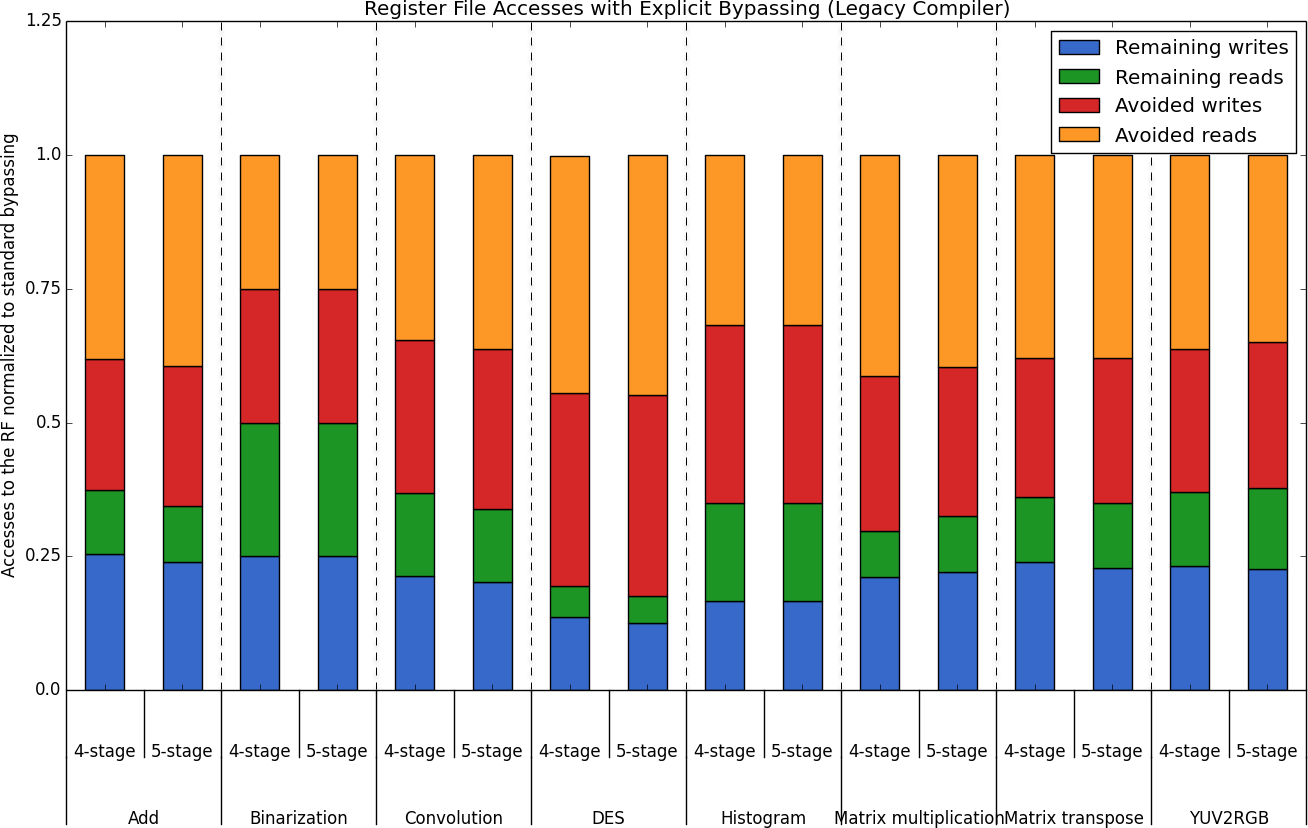
\includegraphics[width=.875\textwidth]{figures/stats/legacy_accesses}
\caption{Register file accesses with explicit bypassing on the legacy compiler (accesses are normalized to the total number of accesses with automatic bypassing) with an overall reduction of at least 50\%, up to 90\% and on average 72\% of write- and 58\% of the read accesses.} %Note that the automatic bypass version does not avoid any write accesses, however it does avoid some read accesses.
\label{fig:legacy_access_improvements}
\end{figure}

This chapter uses the geometric means for averages over normalized statistics (RF accesses and cycle counts). The overall gain by using explicit bypassing are shown in Figure \ref{fig:legacy_access_improvements}, Figure \ref{fig:scalar_improvements} and Figure \ref{fig:vec_accesses} for the legacy compiler, scalar version and vector version of the new compiler respectively. In these figures, the RF accesses performed in the code generated for explicit datapaths are normalized to traditional (implicit) bypassing.





The normalized RF accesses that are performed by the code generated by the legacy compiler is shown in Figure \ref{fig:legacy_access_improvements}. You may observe that there are many bypass opportunities where the most bypass opportunities are found in the \emph{DES} benchmark where it can save roughly 75\% read- and 90\% write accesses, on an absolute of 100k write accesses and 150k read accesses in 100k cycles. Since the RF consumes around 35\% of the total energy, this would lead to an overall energy improvement of an estimated 30\% for that specific benchmark.




\section{Scalar Version Comparison}
This section compares the legacy compiler to the current compiler. It does this by comparing the code generated by the legacy compiler with scalar-only code generated by the current compiler. This gives the following results shown in Figure \ref{fig:legacy_scalar_cmp}. For some benchmarks (\emph{matrix multiplication}) the new compiler has effectively a two times speedup. However, for some benchmarks (\emph{YUV2RGB}) there is actually a decrease in performance. This is caused due to inefficiencies caused by the source-level linker which always adds a \texttt{simm} instruction before using a global variable (even if that is not necessary). Furthermore, the code that the legacy compiler generates for \emph{YUV2RGB} has only three basic block, while the code generated by the new compiler has eighteen basic blocks. The new compiler has a decrease in performance for this benchmark because of this structural overhead. However, the new compiler performs better on average.

%FUUUCK THIS PART, REMOVE IS REQUIRED :(
%Moreover, the legacy compiler does not even generate a correct result for \emph{YUV2RGB}, therefore, it does not matter that the new compiler needs more cycles to complete, because the new compiler does give a correct result.

%up to 50\% (\emph{matrix multiplication}) and 

\begin{figure}[H]
\centering
\hspace*{-.12in}
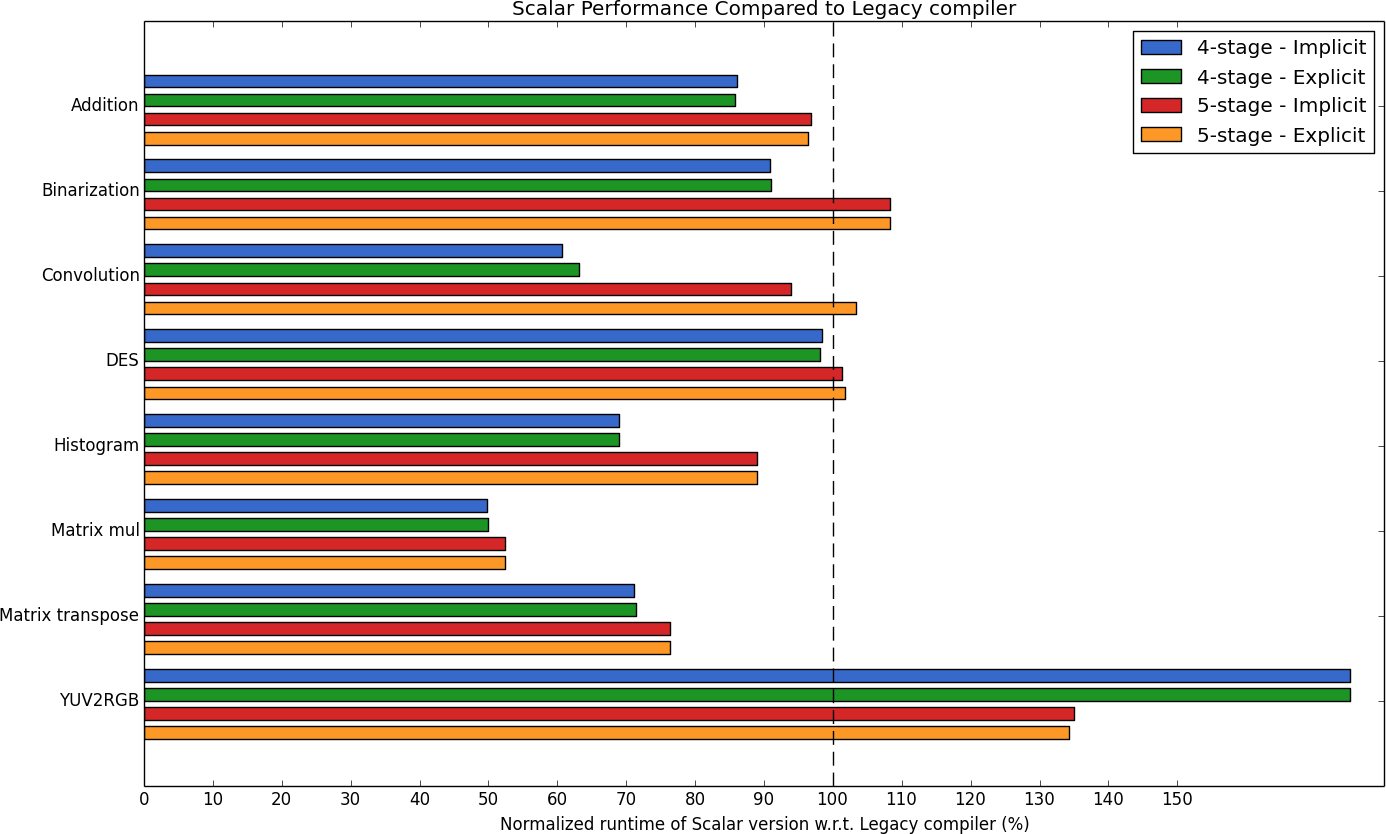
\includegraphics[width=\textwidth]{figures/stats/scalar_cycles}
%TODO: change orange to yellow and yellow to orange in picture. 
\caption{Scalar version performance comparision (where cycle counts are normalized to the legacy compiler) where less than 100\% indicates an improvement and more than 100\% indicates a slowdown compared with the legacy compiler. The average improvement is a reduction of 13.8\% in cycles.}
\label{fig:legacy_scalar_cmp}
\end{figure}

Note the code generated for a five-stage pipeline is always worse than the code generated for a four-stage pipeline, because it is effectively the same code with possibly additional stall cycles inserted when a hazard was encountered by hazard recognizer described in Chapter \ref{sec:hazard_recogn}.

To conclude, the new compiler is overall faster with a reduced execution time of 13.8\% on average (geometric mean) and since power consumption is directly related to energy and execution time, this already gives significant improvements. 

\begin{figure}[t!]
\centering
\hspace*{-.12in}
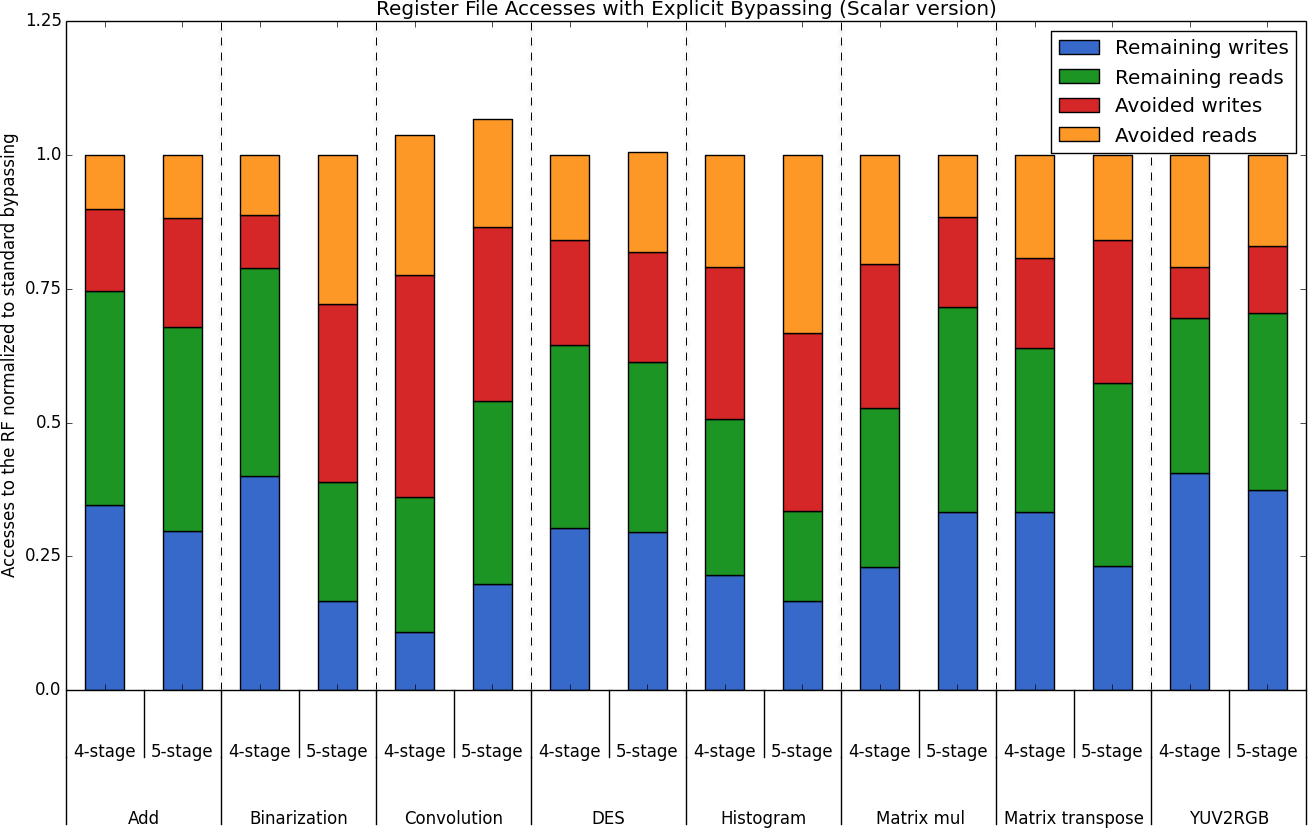
\includegraphics[width=.875\textwidth]{figures/stats/scalar_accesses}
\caption{Scalar version register accesses (RF accesses are normalized to implicit bypassing), with an average reduction of over 42\% on write- and 36\% on read accesses.}
\label{fig:scalar_improvements}
\end{figure}

%TODO add tekst for zero optimization flag with picture below, and make table for few benchies wqith cycle counts and abs accesses both O0 and O3 and maybe legacy.

%==========================
%BEGIN O ZERO - LOWEST OPT
\begin{figure}[b!]
\centering
\hspace*{-.12in}
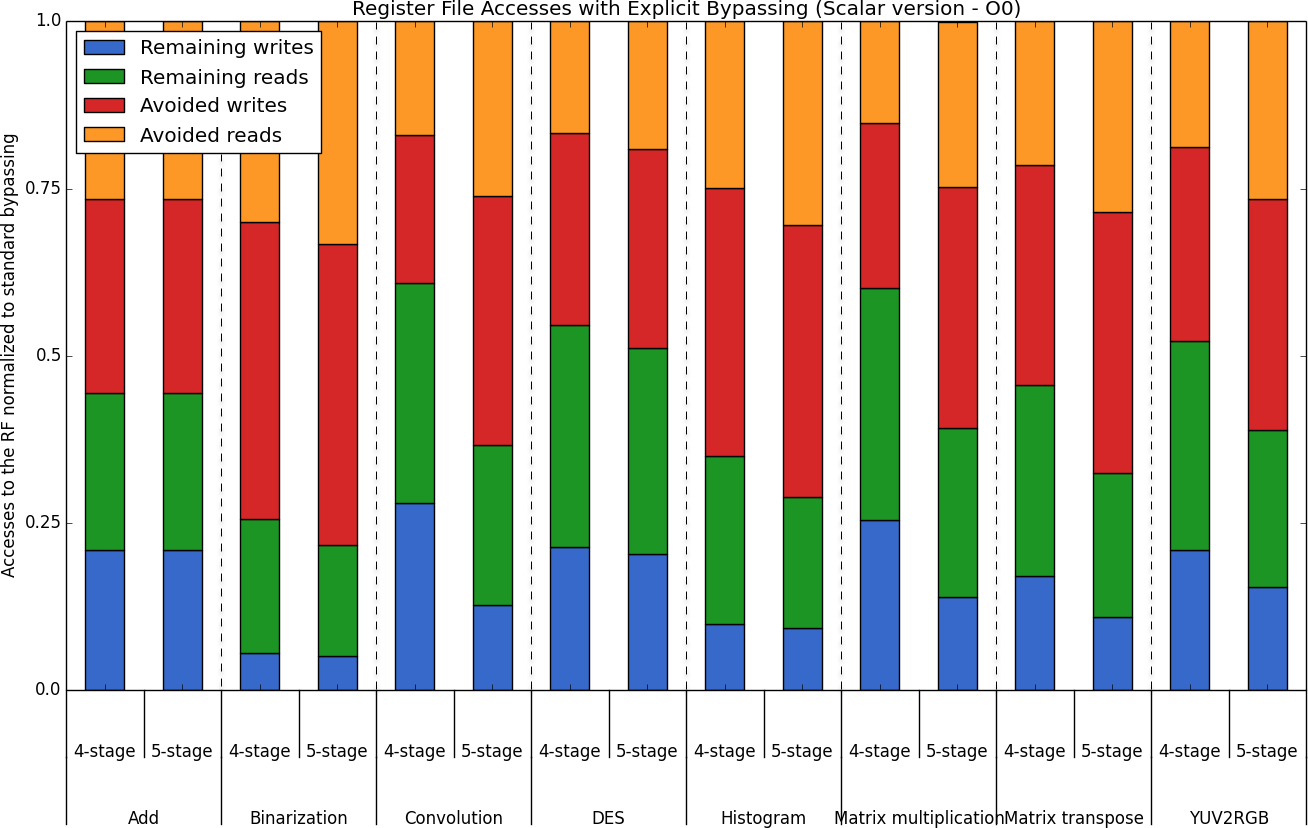
\includegraphics[width=.875\textwidth]{figures/stats/scalar_accesses_O0}
\caption{Scalar version register accesses with opt-level \texttt{-O0} (RF accesses are normalized to implicit bypassing) with an average reduction of 66\% on write- and 45\% on read accesses, and even up to 99.9\% of the write accesses can be avoided.}
\label{fig:scalar_improvements_O0}
\end{figure}

Figure \ref{fig:scalar_improvements} shows a bar chart with how many register file accesses can be avoided with explicit bypassing in the new compiler (accesses are normalized to automatic bypassing). The optimizations for these measurements include optimization level \texttt{-O3} and a scheduler optimization flag, \texttt{-misched-nolimit=1} to limit the scheduling scope and not schedule too far. The instructions are scheduled closer to their use by not buffering instructions during scheduling. The difference in the total number of cycles does not differ compared to \texttt{-O3} with no other optimization flags, but does give an overall improvement in bypass opportunities. There are at least 20\% of the accesses that can be avoided, and up to even 83\% of the writes can be avoided (\emph{convolution}). On average 42\% of the write and 36\% of the read accesses are avoided. Note that convolution jumps over one, which is because that benchmark contains a lot of spill code in the explicit bypass version and the cleanup pass to remove redundant spill code is not implemented yet. Therefore, the explicit version has a significant longer runtime and many more instructions than with standard bypassing and has, therefore, more RF accesses than standard (implicit) bypassing. This can also be seen in Table \ref{table:benchmarks_summary} where it notes that for \emph{convolution} an additional 4000 and 15432 cycles are executed with explicit datapath version of the four-stage and five-stage pipelines respectively.\\

With the lowest optimization level (\texttt{-O0}), the improvement on RF accesses go up to 66\% write- and 45\% avoided read accesses on average. With such low optimization level, the total number of cycles increases rapidly with an increase of up to 6-7 times (convolution). However, for some benchmarks, e.g. histogram, it still performs quite well with only a 50\% increase in cycles, while the increase in utilization of the bypass network is significant (99.9\% write accesses are avoided). Figure \ref{fig:scalar_improvements_O0} shows RF accesses with explicit bypassing, the lowest optimization level and scalar-only code. A large performance lost due to such low optimization level was found for all benchmarks, except for \emph{histogram} and \emph{binarization}. For these two benchmarks which execute in around 50\% more cycles, do have a significant result by avoiding up to almost all write accesses. Table \ref{table:absolute_O0} shows the absolute accesses and cycle counts for these benchmarks. Note that even though a higher latency results from such low optimization flag, the absolute write accesses drastically decreases.


\begin{table}[t!]
\caption{Absolute cycles and accesses for \emph{binarization} and \emph{histogram} with an explicit datapath and five-stage pipeline.}
\begin{center}
\begin{tabular}{@{}l l l l | l l l | l l l@{}}
\toprule
\textbf{Benchmark} 	& \multicolumn{3}{@{}c@{}}{\textbf{Scalar (O3)}}	& \multicolumn{3}{@{}c@{}}{\textbf{Scalar (O0)}} & \multicolumn{3}{@{}c@{}}{\textbf{Legacy}}\\
				& Cycles & Reads & Writes & Cycles & Reads & Writes & Cycles & Reads & Writes \\ \hline
Binarization		& 20816	& 6405	& 3208	& 32022	& 8007	& \textbf{1607}	& 19211	& 8001	& 4805 \\
Histogram			& 8206	& 2053	& 1544	& 12310	& 2055	& \textbf{7}		& 9228	& 2561	& 2052 \\
\bottomrule
\end{tabular}
\end{center}
\label{table:absolute_O0}
\end{table}%

%END O ZERO - LOWEST OPT
%=========================

%OR 

%\begin{figure}[H]
%\centering
%\subfloat[Register write improvements normalized to automatic bypassing.]{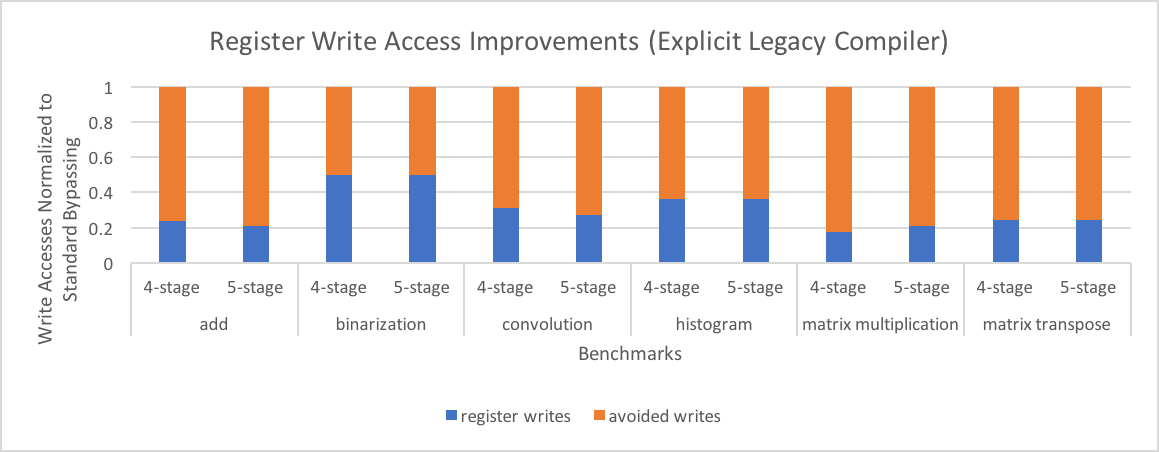
\includegraphics[width=.75\textwidth]{figures/stats/legacy_writes}%
%\label{fig:legacy_write_impr}}
%\hfil
%\subfloat[Register read improvements normalized to automatic bypassing.]{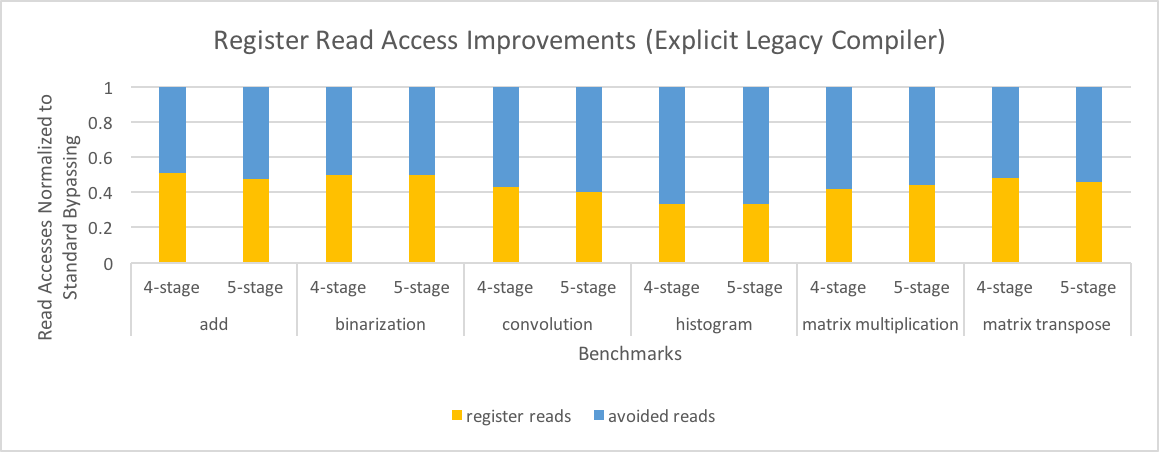
\includegraphics[width=.75\textwidth]{figures/stats/legacy_reads}%
%\label{fig:legacy_read_impr}}
%\caption{Gain in access to the bypass network, normalized to register accesses by the automatic bypass version. }
%\label{fig:legacy_access_improvements}
%\end{figure}
\begin{figure}[b!]
\centering
\hspace*{-.12in}
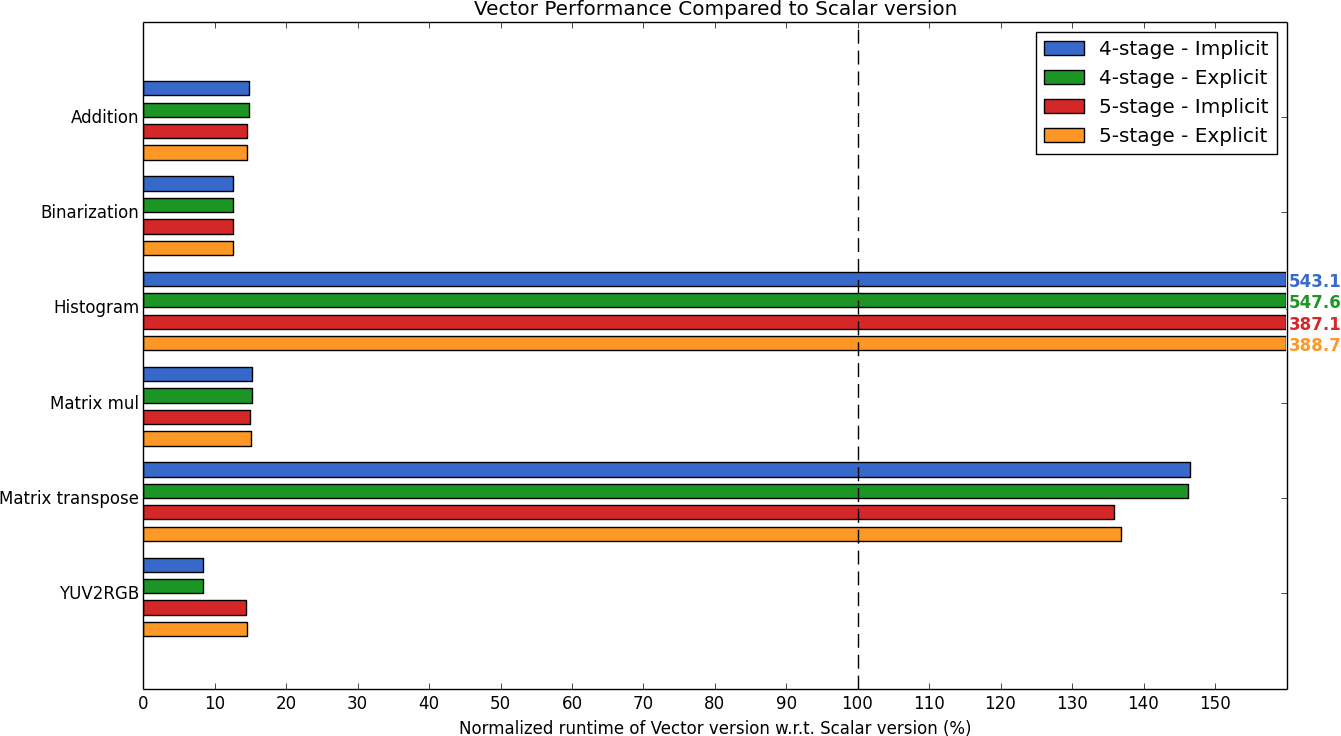
\includegraphics[width=\textwidth]{figures/stats/vector_cycles}
%TODO: change orange to yellow and yellow to orange in picture. 
\caption{Vector version performance gain (cycle counts are normalized to that of the scalar-version), with an average improvement of 65 percent.}
\label{fig:vector_scalar_cmp}
\end{figure}

% ==================================================================
% BEGIN			VECTOR COMPILER ===================================
% ==================================================================
\section{Vector Version Comparison}
The \emph{Data Encryption Standard} (DES) benchmark has not been vectorized because of irregular memory accesses. For other benchmarks e.g. \emph{histogram} and \emph{matrix transpose}, vectorization results in less efficient code. This is often caused by neighborhood network communication which is expensive for the target architecture.

%TODO: ADD PROBLEM OF CONVOLUTION VECTRIZATION, namely !! REDUCTION !!
\emph{Convolution} has not been vectorized because of an open issue with vectorized kernels that use reduction. The \emph{binarization} and \emph{YUV2RGV} benchmarks had some difficulties during vectorization because of a compilation problem when multiple set-flag and conditional move operations are present in a generated code. Problems like these and others are described in the future work section in Chapter \ref{chapter:conclusion}. In overall, the vectorized versions perform better with a maximal obtained speedup of eleven times faster (\emph{YUV2RGB}). However, as already indicated, sometimes, vectorization results in less efficient code, and can cause a four-times slowdown in execution time (histogram). Figure \ref{fig:vector_scalar_cmp} provides an bar chart on which one can see how efficient a benchmark can be vectorized and Table \ref{table:benchmarks_summary} provides an overview with which of the benchmarks are vectorized.

Finally, Figure \ref{fig:vec_accesses} shows the RF accesses with explicit bypassing for the vector versions. With an average around 30\% on write- and over 40\% of read accesses can be avoided. With up to 66\% avoided write accesses (\emph{matrix multiplication}). 

\begin{figure}[t!]
\centering
\hspace*{-.12in}
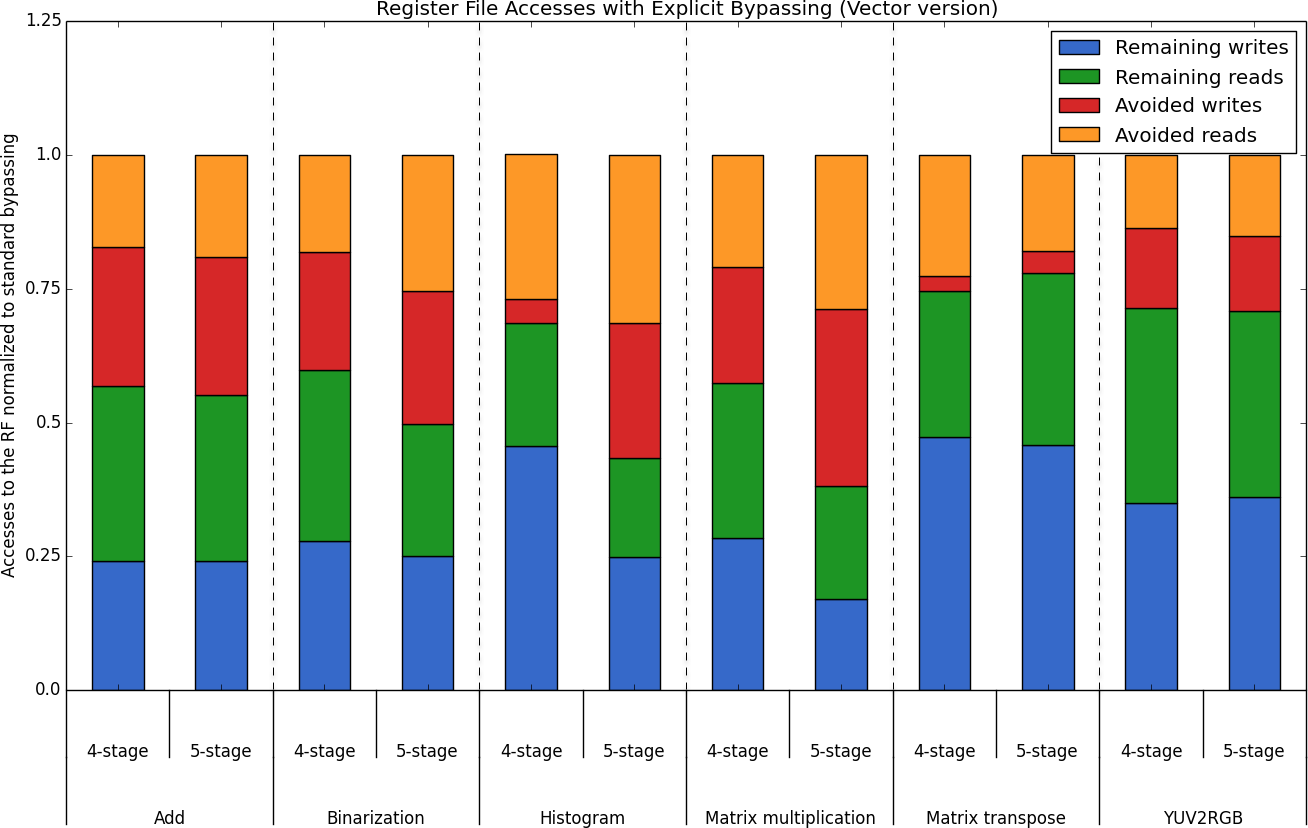
\includegraphics[width=.875\textwidth]{figures/stats/vec_accesses}
%TODO: change orange to yellow and yellow to orange in picture. 
\caption{RF accesses for the vector version, accesses are normalized to standard bypassing.}
\label{fig:vec_accesses}
\end{figure}



%TODO MAKE BELOW USEFUL AND ADD IT :D - xxx me
%\newpage

%Matrix mul benchmark, desired code. Give actual and then desired code! (that is the code below).



%TODO: discuss any inefficiencies here: 
%1: Inefficiencies by the source-level-linked, e.g. always zimm/simm in front of address to a global variable. 
%	This behaviour needs to be implemented by the standard linker too!

%2: Give one full application still needs to be done! :(
%3: discuss or at least think of a way to optimally reduce comm. using DDGs and traits


%\begin{lstlisting}
%A:
%   addi r11, r11, -4 || v.addi r11, r11, -4
%   sw   r10, r11,  0
%   add  r10, r11, r0
%B:
%   lw   r1,  r10,  0
%C:
%   addi r3,  r0,   0 || v.addi r2,  r0,  16
%   lw   r4,  r3,   0 || v.lw   r5,  r2,   0
%   lw   r5,  r3,   1 || v.lw   r4,  r2,   1
%   lw   r6,  r3,   2 || v.lw   r3,  r2,   2
%   lw   r7,  r3,   3 || v.lw   r2,  r2,   3
%D:
%   addi r4,  r4,   0 || v.add  r6,  CP,  r0
%   addi r5,  r5,   0 || v.add  r7,  CP,  r0
%   nop               || v.mul  r6,  r5,  r6
%   nop               || v.mul  r7,  r4,  r7
%   nop               || v.add  r6,  r7,  r6
%   addi r6,  r6,   0 || v.add  r7,  CP,  r0
%   nop               || v.mul  r7,  r3,  r7
%   addi r7,  r7,   0 || v.add  r8,  CP,  r0
%   nop               || v.add  r6,  r7,  r6
%   nop               || v.mul  r7,  r2,  r8
%   nop               || v.add  r6,  r7,  r6
%   addi r1,  r1,  -1 || v.addi r7,  r0,  32
%   sfeq r1,  0       || v.sw   r6,  r7,   0
%   bf   E
%   nop
%   j    C  
%   nop
%E:
%   lw   r10, r11,  0
%   addi r11, r11,  4 || v.addi r11, r11,  4
%   jr r9
%   nop
%\end{lstlisting}